\subsection{Algorytm identyfikacji autorstwa tekstu}

Do wielogłowicowej sieci wprowadzamy w jednym momencie teksty wielu autorów, pochodzących ze zbioru 
testowego w postaci paczek danych (batche). Oprócz danych moduł batchowania dostarcza również 
oczekiwanie wyjście, które posłuży do obliczania wartości funkcji kosztu oraz ewaluacji skuteczności. 
Sieć składa się z określonej przez parametr liczby warstw ukrytych oraz warstw wyjściowych, 
liniowych (tzw. głowic), które predykują rozkład prawdopodobieństwa dla kolejnego znaku. 
W tym celu na danych wyjściowych na każdej głowicy liczona jest funkcja softmax. 
Następnie wykorzystując
krosentropię wyliczany jest koszt, który odzwierciedla jak bardzo jeden rozkład 
prawdopodobieństwa opisuje drugi rozkład. Następnie koszty, które nie ``należą'' do danej głowicy są wygaszane maską. Chodzi o to, by 
każda głowica uczyła się tylko na tekstach swojego autora. Z niewygaszonych kosztów liczona jest średnia.
Po przeprowadzeniu podobnego procesu na wszystkich głowicach oraz po przejściu całego batcha
 dokonywana jest propagacja wsteczna. 
Z wykorzystaniem algorytmu optymalizacji Adam uaktualniane są wagi. Proces szkolenia sieci
możemy więc określić jako uczenie głowic predykcji kolejnych znaków dla swojego autora na podstawie
danych wyjściowych z rekurencyjnych warstw, natomiast proces identyfikacji autorstwa jest szukaniem głowicy, 
która najlepiej predykuje znaki dla nieznanego autora.

\begin{figure}[H]
\centering
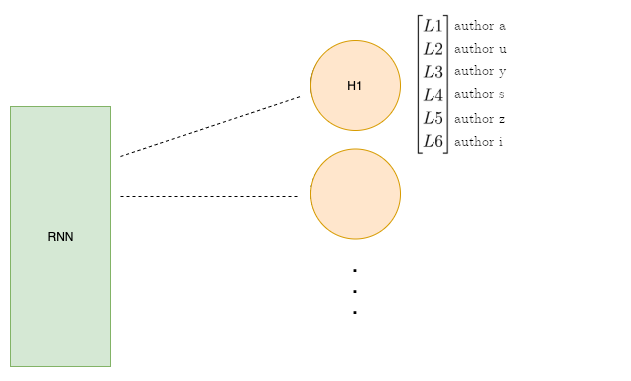
\includegraphics[height=7cm]{./images/rnn-output-2.png}
\caption{Przykładowe wyjście z głowicy numer 1 (Ln - litery).}
\label{fig:test5}
\end{figure} 

Do badania skuteczności sieci wykorzystywany jest zbiór walidacyjny. Do modelu wprowadzane są dane, 
następnie otrzymane wyniki są sprowadzane do wartości z przedziału [0,1], 
gdzie wynik bliski 1 oznacza najmniej pasującego autora, a bliski 0 najbardziej dopasowanego.
Dzięki temu możemy stwierdzić, którego autora przewiduje sieć i zestawić to z prawdziwym wynikiem.
Skuteczność opisana jest jako stosunek poprawnych odpowiedzi do wszystkich. Niska skuteczność może 
świadczyć o źle dobranych parametrach sieci bądź niepoprawnie przeprowadzonym procesie uczenia.